%! TeX program = xelatex

\documentclass[12pt, a4paper]{article}
\usepackage{cmap}
\usepackage[fontsize=12pt]{scrextend}
\usepackage[T2A]{fontenc}
\usepackage[utf8]{inputenc}
\usepackage[english,russian]{babel}
\usepackage{amsmath,amsfonts,amssymb,amsthm,mathtools}
\usepackage[left=20mm, top=20mm, right=20mm, bottom=20mm, nohead, footskip=1cm]{geometry}
\usepackage{multirow}
\usepackage{array}
\usepackage{multicol}
\usepackage{graphicx}
\usepackage{wrapfig}
\usepackage{indentfirst}
\usepackage{enumitem}

\usepackage{polyglossia}
\usepackage{titlesec}
\usepackage{sectsty}
\usepackage{setspace}
\usepackage{fontspec}
\defaultfontfeatures{Mapping=tex-text}

\usepackage{lipsum}
\usepackage{tocloft}
\usepackage[dvipsnames]{xcolor}

\usepackage{caption}
%\captionsetup{labelfont=it, textfont=it}
%\captionsetup[figure]{name=Схема}

\usepackage{hyperref}

\hypersetup{
    colorlinks=false,
    linktoc=all
}
\urlstyle{same}

\setmainlanguage{english}
\setotherlanguage{russian}
\setkeys{russian}{babelshorthands=true}
\setmainfont{Times New Roman}
\newfontfamily\cyrillicfont{Times New Roman}
%\let\cyrillicfonttt\ttfamily
%\onehalfspacing

%\allsectionsfont{\centering}
\renewcommand{\cftsecleader}{\cftdotfill{\cftdotsep}}

%======================================SECTIONING=========================================
%\makeatletter
%\renewcommand*\l@section{\@dottedtocline{1}{1.5em}{2.3em}}
%\makeatother
%======================================SECTIONING=========================================

\pretolerance=6000
\tolerance=3000
\emergencystretch=4pt

\setlength\intextsep{10pt}

\graphicspath{{./visuals/}}
\setlength{\parskip}{0.3125cm}
\setlength{\parindent}{1.25cm}
\setlength{\columnsep}{1cm}
\author{Grigoryev Mikhail}
\title{Algs lab}

\begin{document}

\thispagestyle{empty}

\vspace{30mm}

\begin{center}
FEDERAL STATE AUTONOMOUS EDUCATIONAL INSTITUTION \\
OF HIGHER EDUCATION \\
ITMO UNIVERSITY

\vspace{40mm}

{\large \textbf{Report \\
on the practical task No. 8 \\
"Practical analysis of advanced algorithms."}}
\end{center}

\vspace{15mm}

\begin{flushright}
{\large Performed by \\
\textit{Mikhail Grigoryev (370852) \\
Semenova Valeria (370061) \\
Academic group J4133c \\}
Accepted by \\
Dr Petr Chunaev}
\end{flushright}

\vspace{80mm}

\begin{center}
St. Petersburg \\
2022
\end{center}

\newpage

\section*{Goal}
\addcontentsline{toc}{section}{Goal}

Practical analysis of advanced algorithms.

\section*{Formulation of the problem}
\addcontentsline{toc}{section}{Formulation of the problem}

Choose two algorithms not considered in the course from the selected sections of the book \textit{Introduction to algorithms} by \textit{Thomas H. Cormen et. al.}, implement them and produce experiments on them considering their time and space complexity. Analyze the results of experiments as well as theoretical foundations of the algorithms.

\section*{Brief theoretical part}
\addcontentsline{toc}{section}{Brief theoretical part}

The two chosen algorithms from the chapter \textit{Minimum Spanning Trees} were Kruskal's and Prim's algorithms of finding Minimum Spanning Trees of undirected weighted graphs.

\newpage

\section*{Results}
\addcontentsline{toc}{section}{Results}

Aboba.

\begin{figure}[!h]
\centering
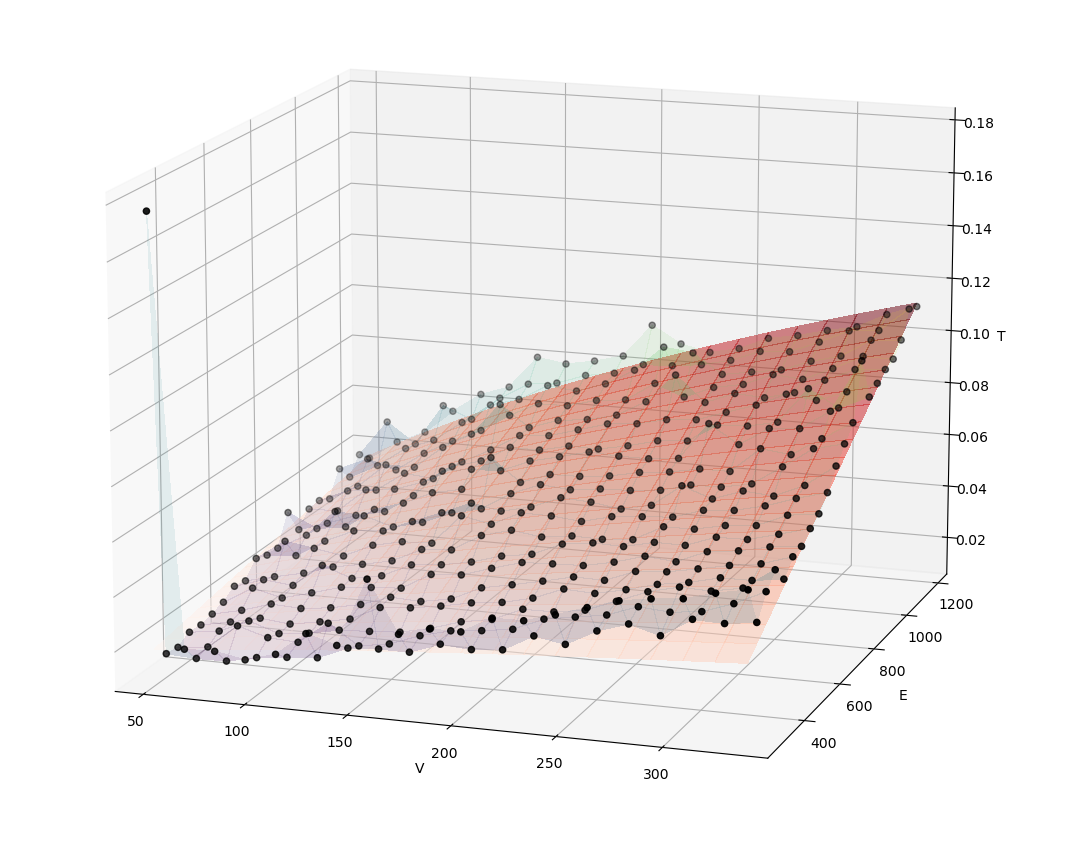
\includegraphics[width=0.49\textwidth]{kruskal_1.png}
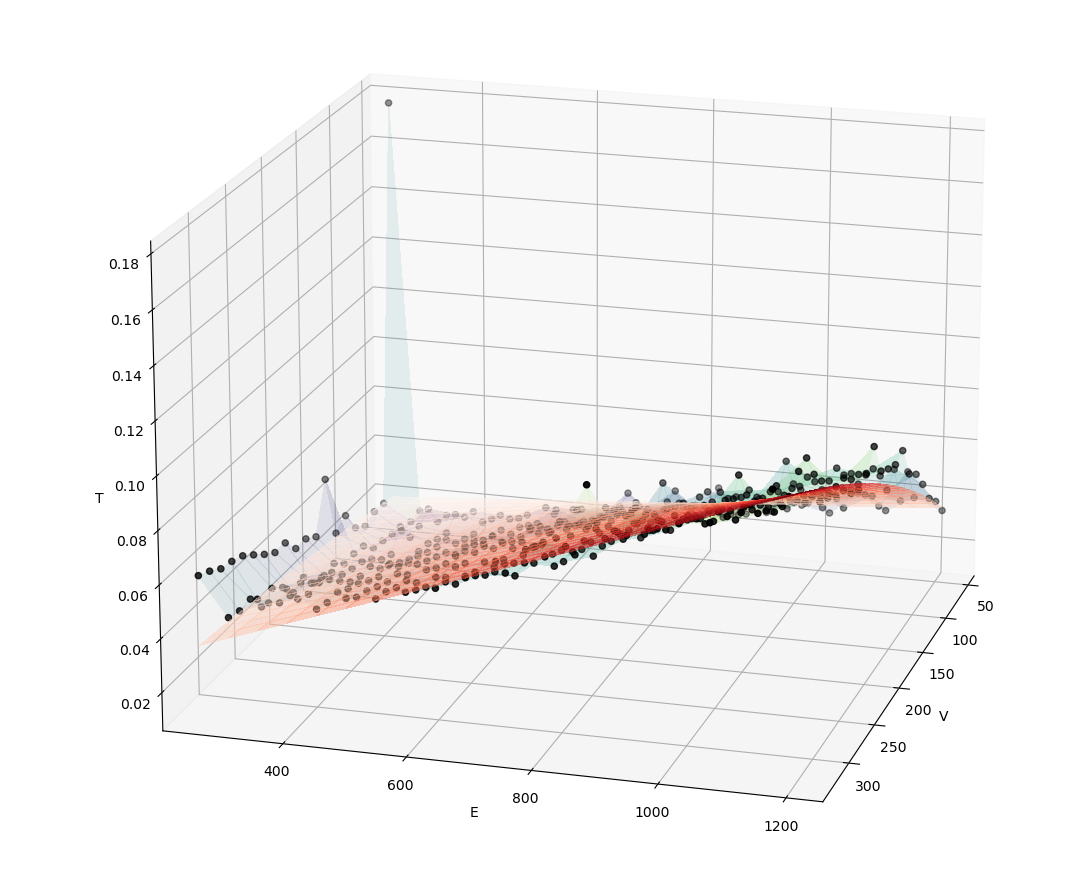
\includegraphics[width=0.49\textwidth]{kruskal_2.png}
\caption{Theoretical time complexity surface fitted on experimental runtimes for Kruskal's algorithm.}
\end{figure}

\begin{figure}[!h]
\centering
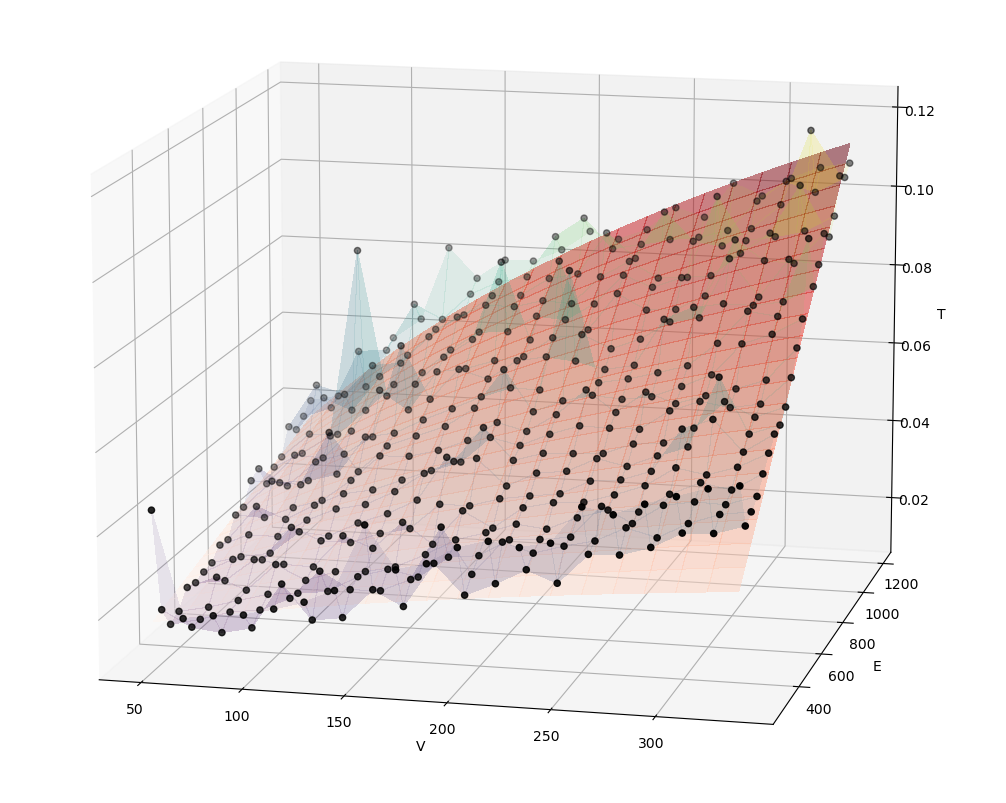
\includegraphics[width=0.49\textwidth]{prim_1.png}
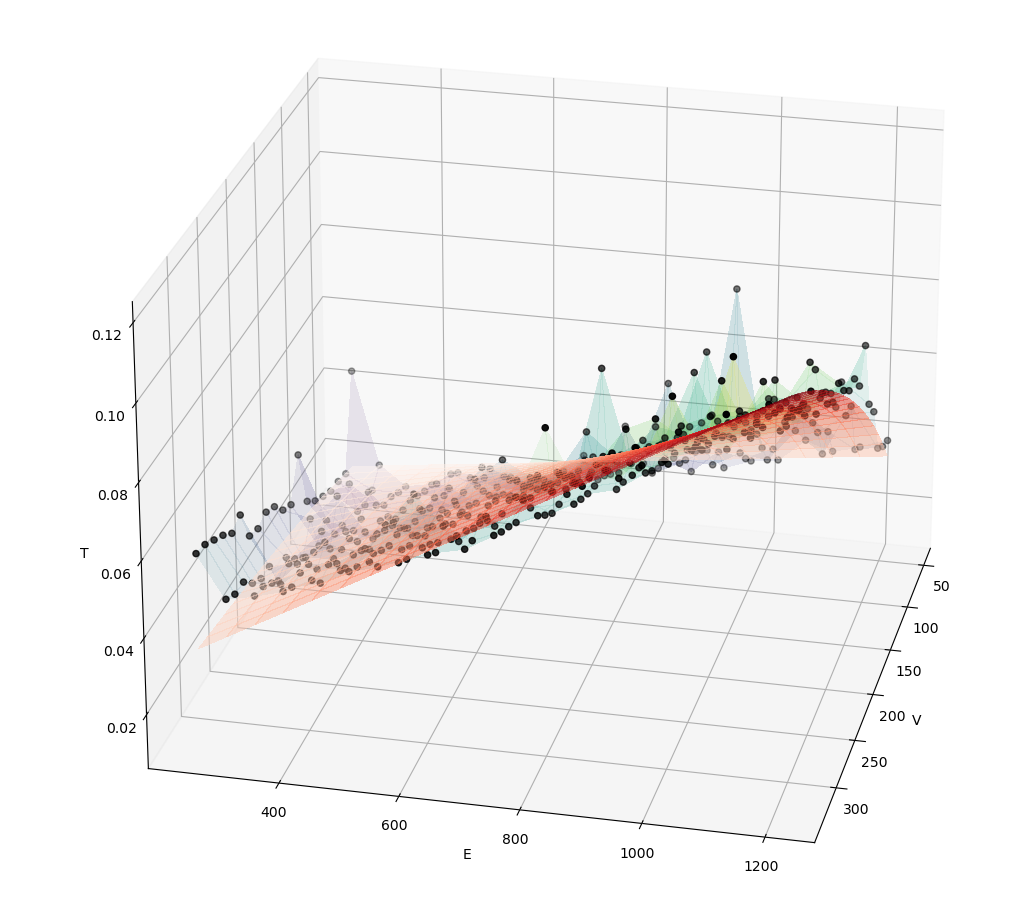
\includegraphics[width=0.49\textwidth]{prim_2.png}
\caption{Theoretical time complexity surface fitted on experimental runtimes for Prim's algorithm.}
\end{figure}

\section*{Conclusions}
\addcontentsline{toc}{section}{Conclusions}

Aboba.

\section*{Appendix}
\addcontentsline{toc}{section}{Appendix}

GitHub link: \url{https://github.com/Dormant512/itmo_lab_listings/blob/main/lab8.py}.

\begin{figure}[!h]
\centering

\includegraphics[width=0.25\textwidth]{lab8.png}
\end{figure}


\end{document}
